\begin{document}
For a better understanding of the data we performed a basic statistical analysis with some variables we found relevant. Some variables have been discarded because they do not provide useful information.% like for example the IDs.

\subsection{Numerical variables}
The following table presents a summary of basic statistical indicators for the numerical variables:

\begin{table}[h!]
\centering
\begin{tabular}{||c c c c c c c c||} 
 \hline
 \textbf{Variable name} & \textbf{Min}  & \textbf{1st Qu} &\textbf{Median} & \textbf{Mean} & \textbf{3rd Qu} & \textbf{Max} & \textbf{Sd} \\ [0.5ex] 
 \hline\hline
 int\_corr & -0.7000 & -0.0200 &  0.2100 &  0.1948 &  0.4300 &  0.9000 & 0.3076232 \\
 age & 21.00 &  24.00 &  26.00 &  26.09  & 28.00 &  39.00 & 3.353241 \\
 age\_o & 21.00 &  24.00 &  26.00 &  26.1  & 28.00 &  39.00 & 3.358056 \\
 diff\_age & 0.00 &  1.00 &  3.00 &  3.592  & 5.00 &  17.00 & 2.866799 \\
 order & 0.000 & 4.000 & 8.000 & 8.875 & 13.000 & 21.000 & 5.399698 \\
 round & 6.00 & 16.00 & 18.00 & 16.84 & 19.00 & 21.00 & 4.10614 \\
 pf\_o\_amb &  0.000 &  5.000 & 10.000 &  9.486 & 15.000 & 36.000 & 6.135659 \\
 pf\_o\_att & 0.00 &  15.00 &  20.00 &  23.72 &  30.00 & 100.00 & 13.73557 \\
 pf\_o\_sin &   0.00 &  11.75 &  20.00 &  17.38 &  20.00  & 40.00 & 7.633928 \\
 pf\_o\_int & 0.00 &  18.00 &  20.00 &  21.21 &  25.00 &  50.00 & 8.014568 \\
 pf\_o\_fun  & 0.00  & 12.00 &  18.00 &  17.18 &  20.00 &  45.00 & 6.783696 \\
 pf\_o\_sha & 0.00 &  5.00 &  10.00 &  11.02 &  15.00  & 30.00 & 6.667148 \\
 attr\_o & 0.00 &  14.00 &  16.00 &  15.58 &  18.00  & 40.00 & 3.928395 \\
 amb\_o & 0.00 &  15.00 &  17.00 &  17.57 &  19.00  & 50.00 & 3.920065 \\
 sinc\_o & 0.0 &   17.0  &  18.0  &  18.3  &  20.0  &  39.0 & 3.594274 \\
 func\_o & 0.00 &  15.00 &  17.00 &  16.05 &  18.00 &  53.00 & 3.440163 \\
 intel\_o & 0.00 &  17.00 &  18.00 &  19.01  & 20.00 &  50.00 & 3.337487 \\
 shar\_o & 0.00 &  11.00 &  14.00 &  13.72 &  17.00 &  40.00 & 4.280074 \\
 mn\_sat &  0.0 & 0.0 & 1100.0 &  727.3 & 1365.0 & 1490.0 &  661.1259 \\
 like & 1.000 &  5.000 &  6.000 &  6.135 &  7.000 & 10.000 & 1.829171 \\
 income & 8607 &  31432 &  43664 &  45892 &  55080 & 109031 & 17809.83 \\
 imprelig & 1.000 &  1.000 &  3.000 &  3.805 &  6.000 & 10.000 & 2.8707 \\
 imprace & 1.000 &   1.000 &  3.000 &  3.589 &  6.000 & 10.000 & 2.807687 \\
 tuition &  0  & 0 &  12900 &  12384 &  26019 &  34300 & 12093.88 \\
 \hline
\end{tabular}
\caption{Qualitative variables raw information}
\label{table:1}
\end{table}

Now we will analyze the qualitative variables which have useful information in order to achieve our goal of extracting knowledge from the data:
\newpage
\texttt{IMPORTANCE OF RACE}

\begin{figure}
  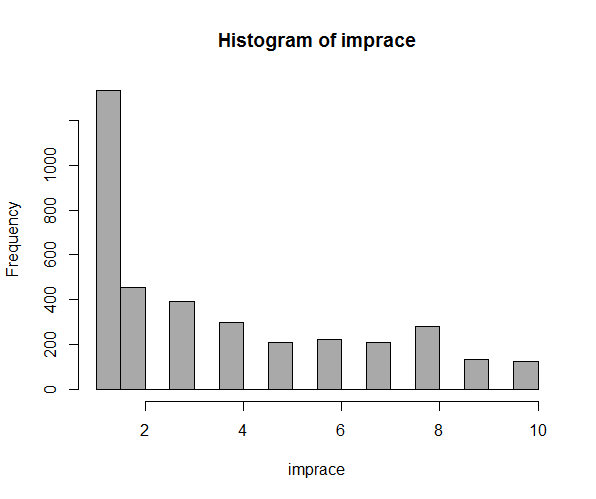
\includegraphics[height=9cm, width=13cm]{images/Hist_Plots_Analysis/hist_imprace.png}
  \caption{Frequency of the importance of the race on dates.}
  \label{fig:imprace}
\end{figure}

In Figure 1 we can see the frequency of the mark that people give to the importance of the race of the partner on a date. The mark is an integer between 1 and 10. And as we can see, most of the people give very little importance to race. The most voted mark by far is a 1. 

\newpage
\texttt{INCOME}

\begin{figure}
  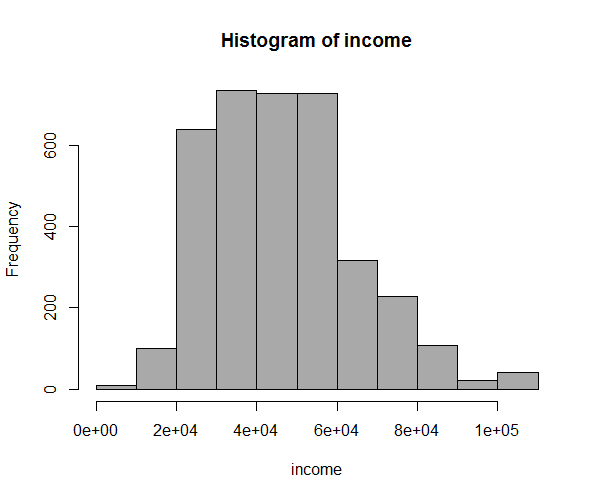
\includegraphics[height=9cm, width=13cm]{images/Hist_Plots_Analysis/hist_income.png}
  \caption{Frequency of the income variable.}
  \label{fig:imprace}
\end{figure}

In Figure 2 we can see the frequency of people income. Most people earn between 40.000\$ and 60.000\$ a year but there is a big difference between the higher and the lower income, the standard deviation is pretty high (17.000\$). We can relate this to people who have studies and people who don't.

\newpage
\texttt{LIKE}

\begin{figure}
  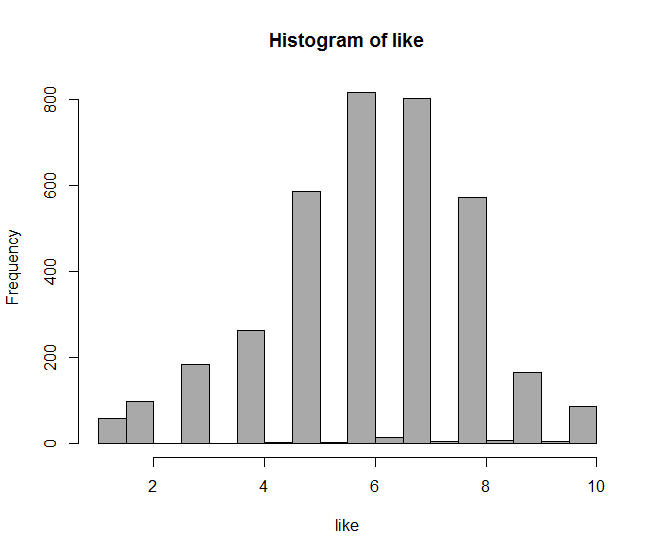
\includegraphics[height=9cm, width=13cm]{images/Hist_Plots_Analysis/hist_like.png}
  \caption{Frequency of the like variable.}
  \label{fig:imprace}
\end{figure}

In Figure 3 we can see the frequency of people voting how much they liked his partner. People tend to vote positively.

\begin{center}
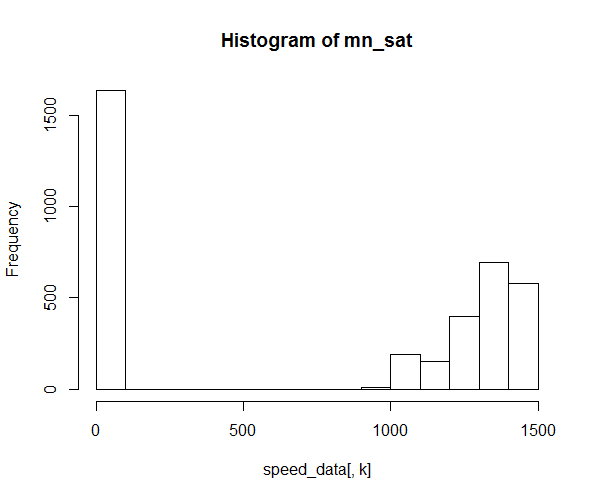
\includegraphics[width=3.5in]{images/Hist_Plots_Analysis/hist_mn_sat.png}
\captionof{figure}{Histogram of mn\_sat.}
\label{fig:aLabelForReferencing}
\end{center}

\begin{center}
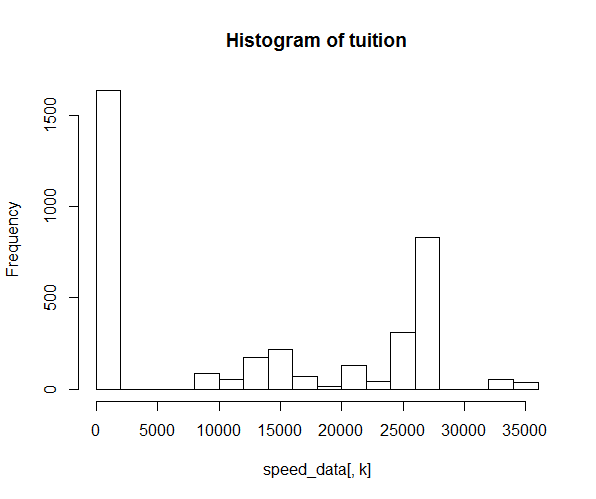
\includegraphics[width=3.5in]{images/Hist_Plots_Analysis/hist_tuition.png}
\captionof{figure}{Histogram of tuition.}
\label{fig:aLabelForReferencing}
\end{center}

As we can see on Figures 5 and 6, this variables have been affected by preprocessing due to most of values are zeros. This is because we transformed all missing values to zeros. We assumed that a missing value meant that the person hasn't gone to university so his mn\_sat and tuition value are zero. Considering that we can appreciate that mm\_sat average is between 1000 and 1500 and that tuition have a peek on 27.500.

\subsection{Categorical variables}

\begin{center}
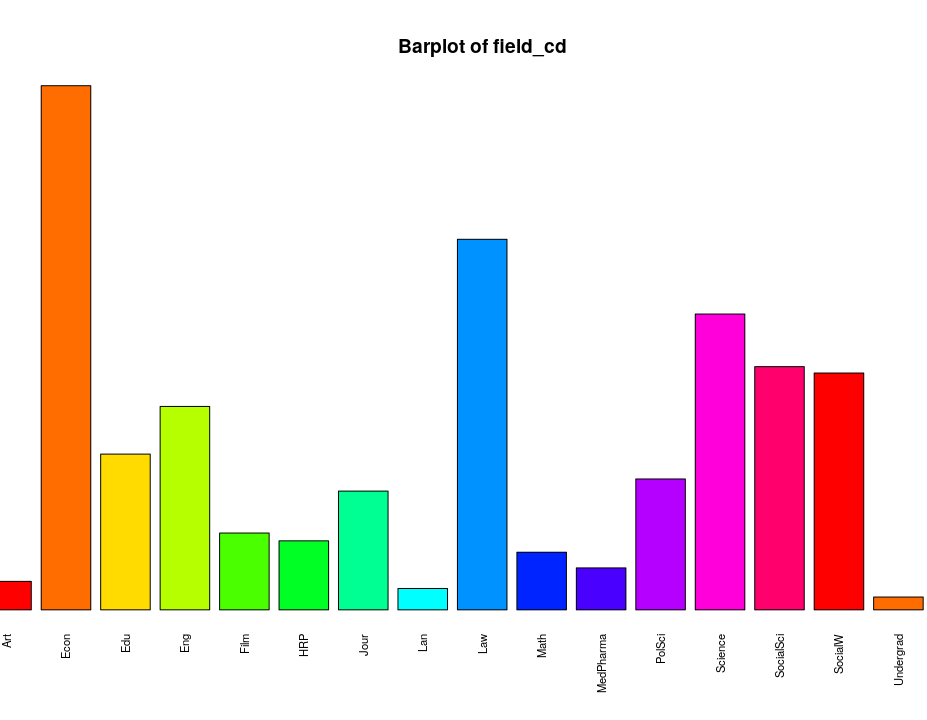
\includegraphics[width=4.5in]{images/Hist_Plots_Analysis/barplot_field_cd.png}
\captionof{figure}{Barplot of people jobs.}
\label{fig:aLabelForReferencing}
\end{center}

\texttt{FIELD\_CD}\\
In Figure 7 we can appreciate the frequency of the occupation of the people who have been dating. With this information we can relate if the occupation of the partner has a big impact on the decision of matching.

\begin{center}
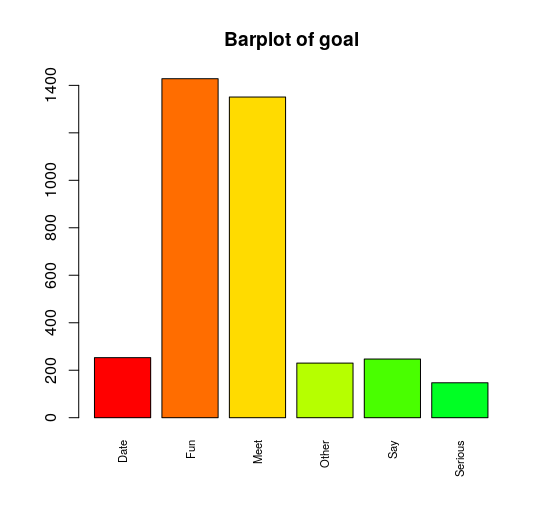
\includegraphics[width=3.5in]{images/Hist_Plots_Analysis/barplot_goal.png}
\captionof{figure}{Frequency of the goal of a date.}
\label{fig:aLabelForReferencing}
\end{center}

\texttt{GOAL}
In Figure 8 we can see the frequency what are the people looking on a date.

\begin{center}
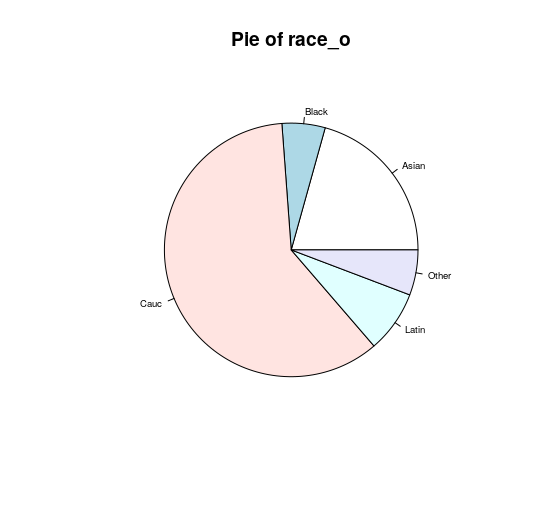
\includegraphics[width=3.5in]{images/Hist_Plots_Analysis/qu3esito_race_o.png}
\captionof{figure}{Race information.}
\label{fig:aLabelForReferencing}
\end{center}

\texttt{RACE}
In figure 9 we can appreciate the frequency of different people races. The majority of the people on this programme are Caucassian. We can relate this variable to the chances of getting a match of every different race.


%\begin{figure}
 % 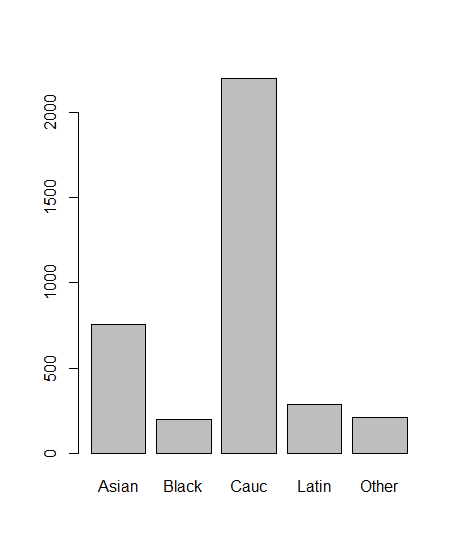
\includegraphics[height=9cm, width=13cm]{images/Hist_Plots_Analysis/plot_race_o.png}
 % \caption{Race\_o information.}
  %\label{fig:boat1}
%\end{figure}


\subsection{Bivariate analysis}

In order to answer the main question of this project, we want to relate the variable \textit{match} with the variables that have more information on giving us an answer to out main question.

\begin{center}
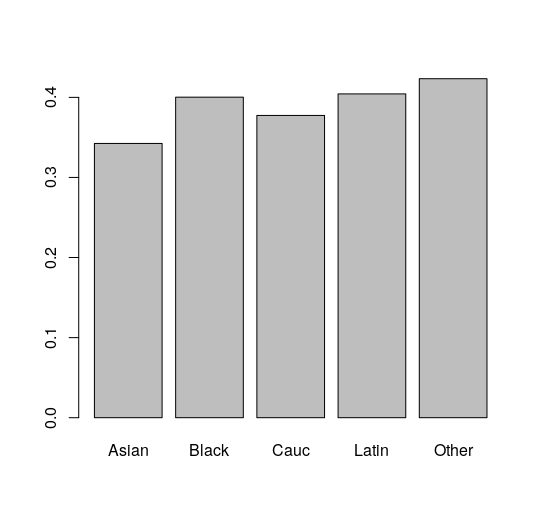
\includegraphics[width=3.5in]{images/Hist_Plots_Analysis/bivar_match_race.png}
\captionof{figure}{Relation between match and race.}
\label{fig:aLabelForReferencing}
\end{center}

As we can see on Figure 10 the race of the people on a date does not seem to have a big impact on having a match, Asians have a slightly difference of matching but overall it is equal.

\begin{center}
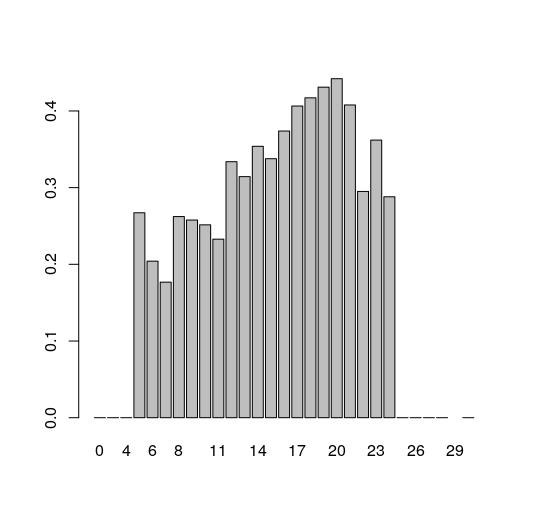
\includegraphics[width=3.5in]{images/Hist_Plots_Analysis/bivar_match_fun_o.png}
\captionof{figure}{Relation between match and fun\_o.}
\label{fig:aLabelForReferencing}
\end{center}

In Figure 11 we can appreciate that people who are more fun on the point of view of their partner have more chances of getting a match that people who have less points on being fun.

\begin{center}
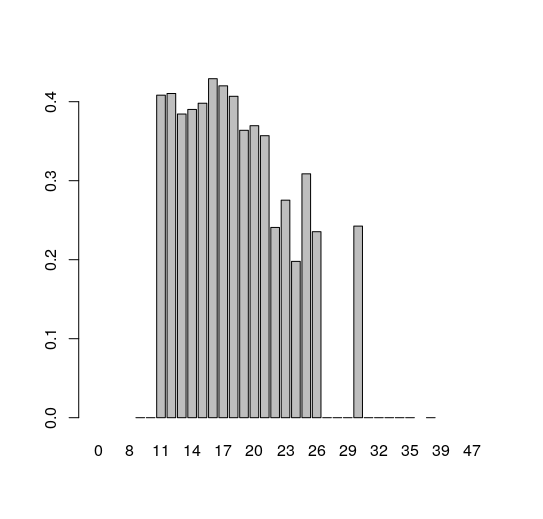
\includegraphics[width=3.5in]{images/Hist_Plots_Analysis/bivar_match_intel.png}
\captionof{figure}{Relation between match and intel\_o.}
\label{fig:aLabelForReferencing}
\end{center}


In Figure 12 we can see that if someone sees you intelligent then a match is less probable. People with low points on intelligent tend to have more matches.



\begin{center}
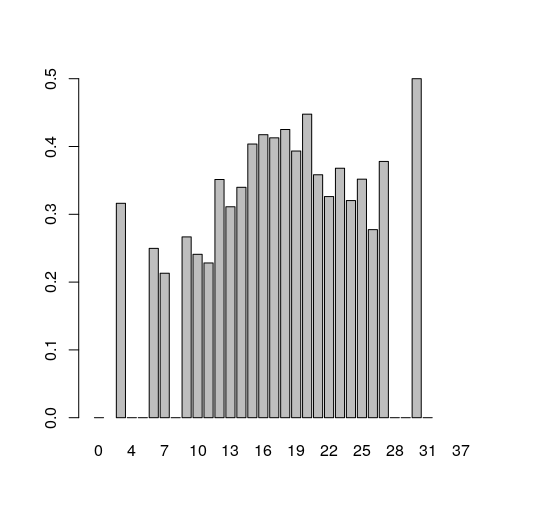
\includegraphics[width=3.5in]{images/Hist_Plots_Analysis/bivar_match_attr.png}
\captionof{figure}{Relation between match and attr\_o.}
\label{fig:aLabelForReferencing}
\end{center}

In figure 13 we can observe that the outliers are very clear, people with very few points in attractiveness have very small chances of getting a match and on the other hand people with a lot of points on attractiveness have a lot of more chances of getting a match.

\begin{center}
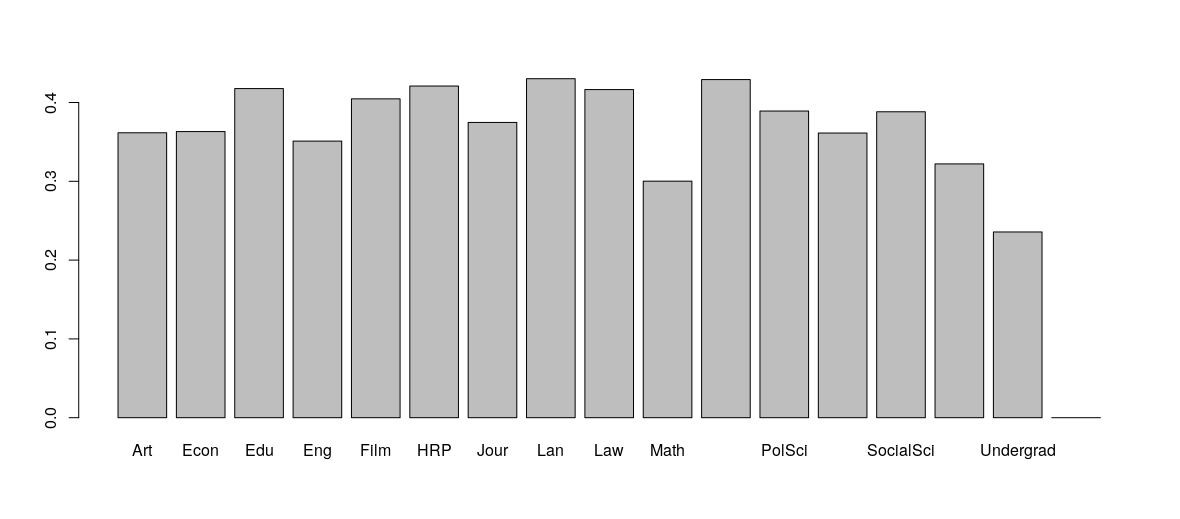
\includegraphics[width=5.5in]{images/Hist_Plots_Analysis/bivar_match_field_cd.png}
\captionof{figure}{Relation between match and field\_cd.}
\label{fig:aLabelForReferencing}
\end{center}

\subsection{How is our data?}
As we said before our data rows represent a date on the point of view of one individual. We want to answer the question "\textit{What features have impact on having a match on SpeedDating}", looking to this first statistical analysis we can conclude that: race is not important on having a match, being fun and attractive to your partner gives you a lot of chances to get the match. But if you seem intelligent you have less opportunities to get the match. Also we concluded that people who work on the field of maths have lower chances of getting a match. Men are more likely to give a positive decision while women do the opposite.

\end{document}